For starting calculations, we will consider the mass of our payload at 100g. Then, the total mass of the rocket is 451g ($ p = \frac{m_p}{m_0} = 0.22 $). For the choice of the engine we used the formula $ T = k \cdot m_0 \cdot g_0 $ , which gives us that the average thrust is between 44.49N and 53.39N.  Thus, we chose the Aerotech D24T-4 engine.

\begin{multicols}{2}

\begin{figure}[H]
\centering
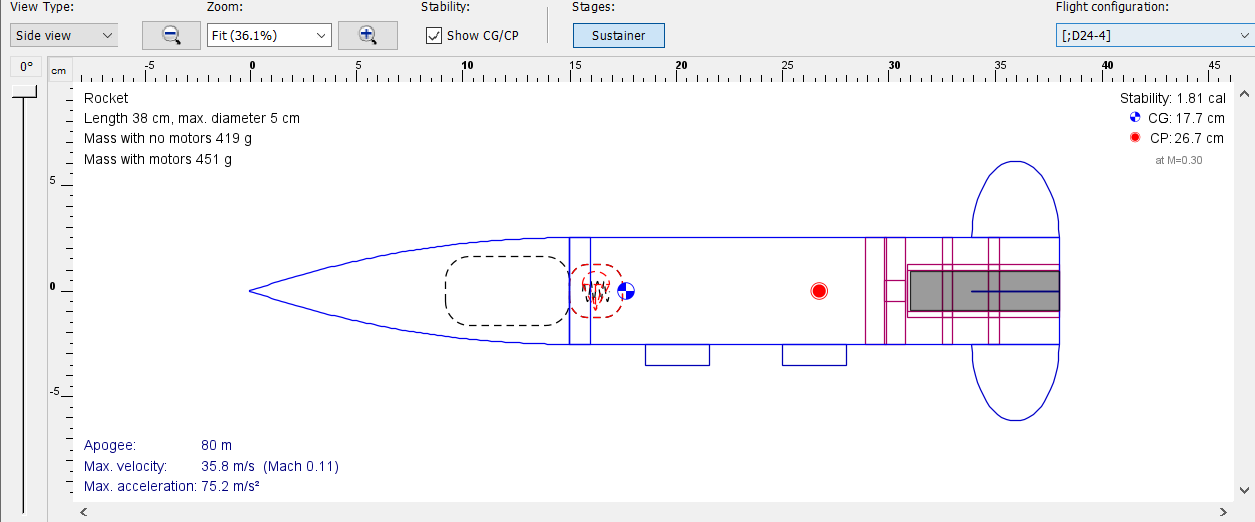
\includegraphics[width=0.8\linewidth]{side_view}
\caption{Side view and details from OpenRocket}
\end{figure}

\begin{figure}[H]
\centering
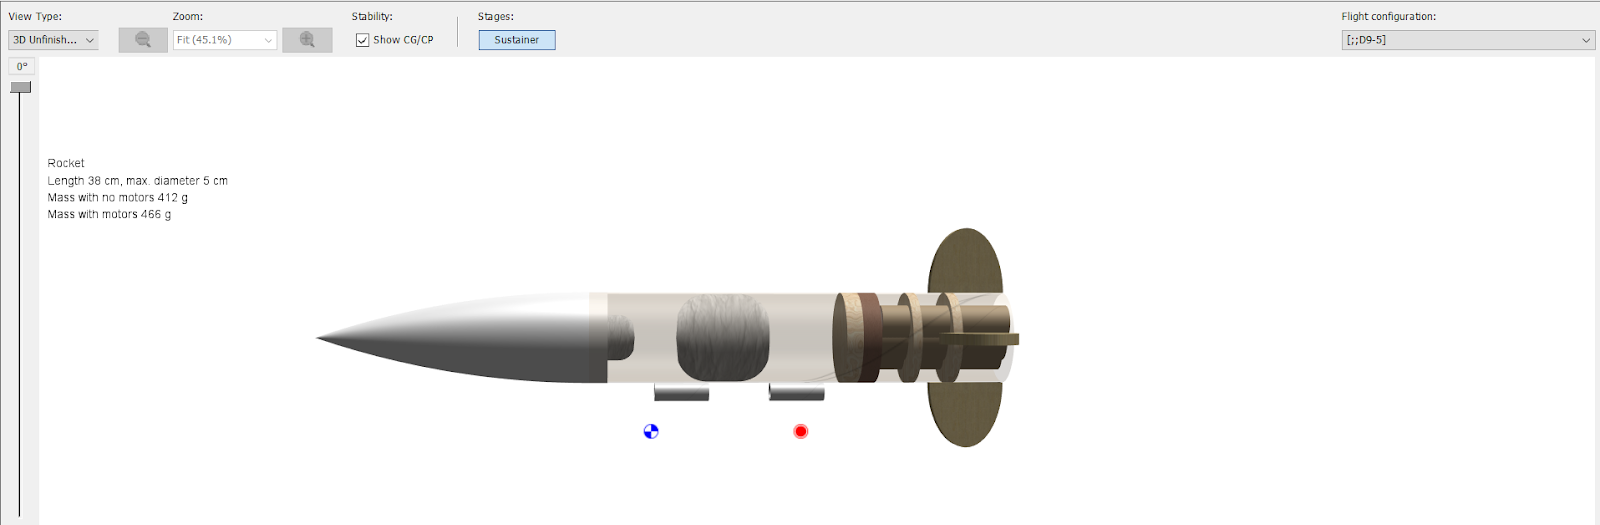
\includegraphics[width=0.8\linewidth]{unfinished_view}
\caption{3D Unfinished view}
\end{figure}

\end{multicols}

\begin{figure}[H]
\centering
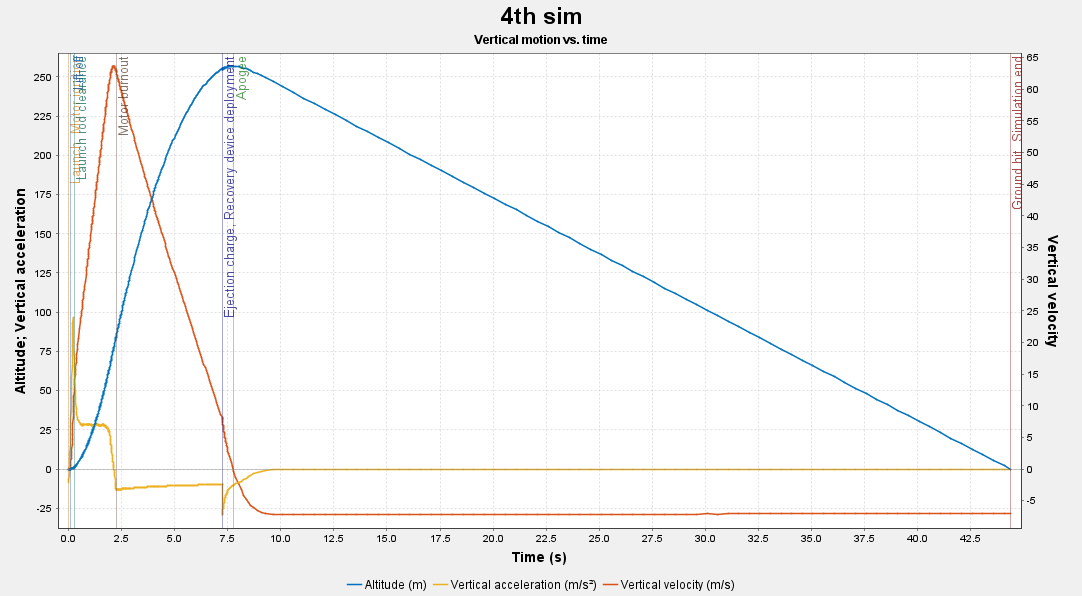
\includegraphics[width=0.5\linewidth]{graph}
\caption{Flight graph}
\end{figure}

Depending on the materials, their densities, properties and roles in 2.2.4. , using the program OpenRocket, we got these next parameters:

\begin{itemize}

\item Length of 380 mm, Diameter of 50 mm; Total Mass 451g, Utile Mass 100g (p=22.17\%);
\item Stability coefficient 1.81; CG 17.7cm; CP 26.7cm;
\item Apogee 80m, max velocity 35.8 m/s, max acceleration $ 75.2 \frac{m}{s^2} $ , optimum delay of 3.45s, flight time 15.6s, ground hit velocity $ 7.46 \frac{m}{s} $;
\item After the simulations we concluded that the optimum diameter of the parachute is 45cm. 

\end{itemize}